 \begin{tcolorbox}
\begin{prop}[Propriedade de Limites] Suponha que c seja uma constante e os limite de $f(x)$ e $g(x)$ existem quando $x$ tende para \textbf{a} então

\begin{enumerate}
\begin{multicols}{2}
    \item $\lim\limits_{x \to a} c\cdot f(x) = c\cdot \lim\limits_{x \to a}f(x)$
    
    \item $\lim\limits_{x \to a} \left(f(x) \pm g(x)\right) = \lim\limits_{x \to a} f(x) \pm \lim\limits_{x \to a}g(x)$
    
    \item $\lim\limits_{x \to a} \left(f(x)\cdot g(x)\right) = \lim\limits_{x \to a} f(x) \cdot \lim\limits_{x \to a}g(x)$
    
    \item $\lim\limits_{x \to a} \left(\dfrac{f(x)}{g(x)}\right)= \dfrac{\lim\limits_{x \to a} f(x)}{\lim\limits_{x \to a}g(x)} \quad \text{se} \quad \lim\limits_{x \to a}g(x)\neq 0$
    \item $\lim\limits_{x\to a}c=c$ \qquad $\lim\limits_{x\to a}x=a$
    \item $\lim\limits_{x\to a}x^n=a^n$, para $n\in \mathbb{Z}^+$
    \item $\lim\limits_{x \to a} \left(f(x)\right)^n = \left(\lim\limits_{x \to a} f(x)\right)^n$, para $n\in \mathbb{Z}^+$
    
    \item $\lim\limits_{x \to a} \left(\sqrt[n]{f(x)}\right)= \sqrt[n]{\lim\limits_{x \to a}f(x)}$ para $n\in \mathbb{Z^{+}}$ (se $n$ é par supomos $\lim\limits_{x\to a}f(x)>0$)
    
\end{multicols}
\end{enumerate}
\end{prop}

\begin{prop}
Todas as propriedades de limites enunciadas na proposição anterior são também válidas para limites laterais.
\end{prop}
\begin{teorema}$\lim\limits_{x \to a}f(x)=L$ se só se  $\lim\limits_{x \to a^-}f(x)=L$ e $\lim\limits_{x \to a^+}f(x)=L$.
\end{teorema}


\subsubsection*{Fatoração e Cancelamento}
\begin{align*}
    \lim\limits_{x \to -3}\dfrac{x^2-x-12}{x^2+3x}=\lim\limits_{x \to -3}\dfrac{(x+3)\cancel{(x-3)}}{x\cancel{(x-3)}}=\lim\limits_{x \to -3}\dfrac{(x-4)}{x}=\frac{7}{3}
\end{align*}
\subsubsection*{Limites Especiais}

\begin{align*}
    \lim\limits_{x \to 0}\frac{\sin(x)}{x}=1, \qquad
    \lim\limits_{x \to 0}\frac{e^x-1}{x}=1
\end{align*}
\end{tcolorbox}
\begin{tcolorbox}
\begin{teorema}[Teorema do Confronto] Se $f(x)\leq g(x)\leq h(x)$ quando $x$ está próximo de $\textbf{a}$ e $\lim\limits_{x \to a}f(x)=L=\lim\limits_{x \to a}h(x)$ então $\lim\limits_{x \to a}g(x)=L$.
\end{teorema}
\begin{figure}[H]
\centering
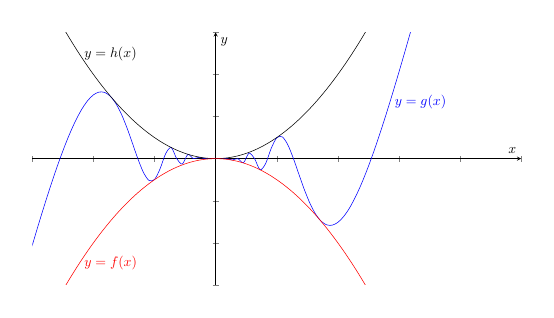
\begin{tikzpicture}[scale=0.5]
\begin{axis}[
 axis lines=middle,
 ticklabel style={fill=white},
 xmin=-1.5,xmax=2.5,
 ymin=-1.5,ymax=1.5,
 xlabel=$x$,ylabel=$y$,
 domain=-2:2.5,
 samples=100,
 smooth, 
 yticklabels={,,},
 xticklabels={,,},
 height=8cm,
 width=14cm]
\addplot[blue] {x*x*sin(4/\x r)}node[pos=0.65,anchor=west]{$y=g(x)$};
\addplot[black] { x*x}node[pos=0.25,anchor=west]{$y=h(x)$};
\addplot[red] {-x*x}node[pos=0.25,anchor=west]{$y=f(x)$};
\end{axis}
\end{tikzpicture}
\end{figure}
\end{tcolorbox}

